\section{30.10.23 : Martyngały}

Mają coś współnego z jazdą konną (podobno).

\begin{example}
  \item Rozważmy dowolną grę i dla uproszczenia niech polega ona na rzucaniu monetą, na której orzeł wypada z $\prob = p \in (0,1)$. Obstawiamy według zasady double or nothing:
    \begin{itemize}
      \item jeśli wypada orzeł, to podwajamy nasz kapitał
      \item jeżeli wypada reszka, to tracimy wszystko
    \end{itemize}
    Czy taka gra jest sprawiedliwa?

    Rozważmy ciąg niezależnych zmiennych losowych $\{\xi_k\}_{k\in\N}$ o tym samym rozkładzie
    $$\prob{\xi_k=2}=1-\prob{\xi_k=0}=p.$$
    Wówczas ciąg
    $$X_n=\xi_n\cdot\xi_{n-1}\cdot...\cdot\xi_1\cdot X_0$$
    reprezentuje stan konta po $n$-tym rzucie, gdzie $X_0$ to jakaś stała.

    Rozważmy $\sigma$-ciało $\set{F}_n=\sigma(\xi_n,...,\xi_1,X_0)$ generowane przez pierwszych $n$ rzutów i stan początkowy. Zadajmy sobie teraz pytanie, ile wynosi
    $$\expected{X_{n+1}}{\set{F}_n}?$$

    Mamy zależność rekurencyjną $X_{n+1}=\xi_{n+1}X_n$, stąd możemy powiedzieć, że
    $$\expected{X_{n+1}}{\set{F}_n}=\expected{\xi_{n+1}X_n}{\set{F}_n}$$
    samo $X_n$ jest w $\set{F}_n$, więc możemy je wyciągnąć przed $\expected$. Dodatkowo, $\xi_{n+1}$ jest niezależne od $\set{F}_n$, więc
    $$\expected{X_{n+1}}{\set{F}_n}=X_n\expected{\xi_{n+1}}{\set{F}_n}=X_n\expected{\xi_{n+1}}=(2p)\cdot X_n$$

    \begin{itemize}
      \item Jeżeli $p>\frac{1}{2}$, to wówczas
        $$\expected{X_{n+1}}{\set{F}_n}\geq X_n$$
        i wtedy taka gra jest korzystna, bo z coraz to kolejnym rzutem oczekiwania rosną.
      \item Jeżeli $p<\frac{1}{2}$, to wówczas
        $$\expected{X_{n+1}}{\set{F}_n}\leq X_n$$
        i gra jest korzystna, ale dla kasyna a nie gracza.
      \item Jeżeli $p=\frac{1}{2}$, to wówczas
        $$\expected{X_{n+1}}{\set{F}_n}=X_n$$
        i w takim przypadku powiemy, że gra jest sprawiedliwa.
    \end{itemize}
\end{example}

Ten ostatni, uczciwy przypadek to jest jeden ze sposobów, na które możemy myśleć o martyngałach.

\begin{definition}[o martyngałach słów kilka]$ $

  \begin{itemize}
    \item Wstępującą rodzinę $\sigma$-ciał
      $$\mathds{F}=\{\set{F}_n\}_{n\in\N},$$
      $\set{F}_n\subseteq \set{F}_{n+1}$, nazywamy \buff{filtracją}
    \item Powiemy, że ciąg zmiennych losowych $\{X_n\}_{n\in\N}$ jest \buff{$\mathds{F}$-adaptowalny}, jeżeli $X_n\in\set{F}_n$.
    \item Adaptowalny i całkowalny ciąg $\{X_n\}$ nazywamy \acc{nadmartyngałem}, jeśli
      $$\expected{X_{n+1}}{\set{F}_n}\leq X_n$$
    \item Adaptowalny i całkowalny ciąg $\{X_n\}$ nazywamy \acc{podmartyngałem}, jeśli
      $$\expected{X_{n+1}}{\set{F}_n}\geq X_n$$
    \item Z kolei ciąg $\{X_n\}$ jest \buff{martyngałem}, jeśli jest jednocześnie nadmartyngałem i podmartyngałem, czyli zachodzi równość
      $$\expected{X_{n+1}}{\set{F}_n}= X_n$$
  \end{itemize}
\end{definition}

\begin{example}
\item Niech $\{\eta_k\}_{k\in\N}$ będą niezależne takie, że $\expected{\eta_k}=0$ dla każdego $k\in\N$. Wówczas jako filtrację możemy rozważyć
  $$\set{F}_n=\sigma(\eta_1,...,\eta_n)$$
  a jako nowy ciąg zmiennych losowych zdefiniujemy jako $M_0=0$ i 
  $$M_n=\sum_{k=1}^n\eta_k.$$
  Tak zdefiniowany ciąg $\{M_n\}$ jest $\mathds{F}=\{\set{F}_n\}$-martyngałem:
  \begin{align*}
    \expected{M_{n+1}}{\set{F}_n}&=\expected{\eta_{n+1}+M_n}{\set{F}_n}=\\
                                 &=\expected{\eta_{n+1}}{\set{F}_n}+\expected{M_n}{\set{F}_n}=\\
                                 &=\expected{\eta_{n+1}}+M_n=0+M_n=M_n
  \end{align*}
\item Dla dowolnej filtracji $\mathds{F}=\{\set{F}_n\}$ i całkowalnej zmiennej losowej $X$ rozważmy
  $$M_n=\expected{X}{\set{F}_n}.$$
  Wówczas
  $$\expected{M_{n+1}}{\set{F}_n}=\expected{\expected{X}{\set{F}_{n+1}}}{\set{F}_n}=\expected{X}{\set{F}_n}=M_n$$
\end{example}

\begin{uwaga}
  Jeżeli $\{X_n\}$ jest martyngałem, to 
  $$\expected{X_{n+1}}{\set{F}_n}=X_n$$
  czyli mam dwie zmienne losowe które są sobie równe, czyli
  $$\expected{X_{n+1}}=\expected{\expected{X_{n+1}}{\set{F}_n}}=\expected{X_n}$$
  W szczególności, jeśli zastosujemy indukcję, to dostaniemy, że dla dowolnego $n\in\N$
  $$\expected{X_n}=\expected{X_0}$$
\end{uwaga}

\begin{example}
\item \buff{Proces Gaultona-Watsona}

  Rozważmy populację, w której osobniki rozmnażają się bezpłciowo, niezależnie od siebie. Można myśleć o tym jako o obserwacji populacji pantofelków z pomiarami w jakiś określonych odstępach czasu.

  Myślimy o tym jako o drzewie, w którym liczba krawędzi z danego wierzchołka oznacza liczbę potomstwa, a ilość wierzchołków na danej głębokości oznacza ilość pantofelków po $n$-tym pokoleniu.

  \begin{center}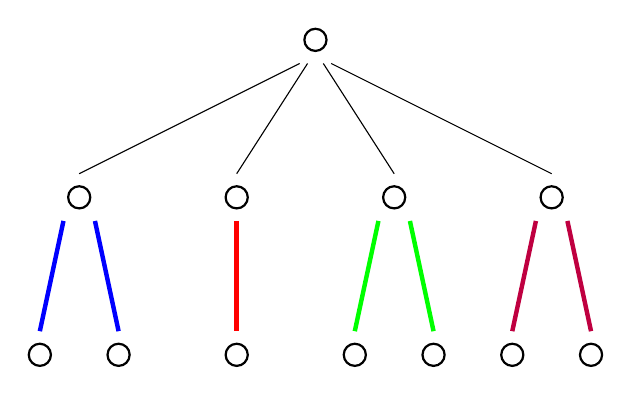
\begin{tikzpicture}
    \draw[thick] (0, 0) circle (4pt);

    \draw (-0.2, -0.3)--(-3, -1.7);
    \draw (-0.1, -0.3)--(-1, -1.7);
    \draw (0.1, -0.3)--(1, -1.7);
    \draw (0.2, -0.3)--(3, -1.7);

    \draw[thick] (-3, -2) circle (4pt);
    
    \draw[blue, ultra thick] (-3.2, -2.3)--(-3.5, -3.7);
    \draw[blue, ultra thick] (-2.8, -2.3)--(-2.5, -3.7);

    \draw[thick] (-3.5, -4) circle (4pt);
    \draw[thick] (-2.5, -4) circle (4pt);


    \draw[thick] (-1, -2) circle (4pt);

    \draw[red, ultra thick] (-1, -2.3)--(-1, -3.7);


    \draw[thick] (-1, -4) circle (4pt);


    \draw[thick] (1, -2) circle (4pt);

    \draw[green, ultra thick] (0.8, -2.3)--(0.5, -3.7);
    \draw[green, ultra thick] (1.2, -2.3)--(1.5, -3.7);

    \draw[thick] (0.5, -4) circle (4pt);
    \draw[thick] (1.5, -4) circle (4pt);


    \draw[thick] (3, -2) circle (4pt);

    \draw[purple, ultra thick] (2.8, -2.3)--(2.5, -3.7);
    \draw[purple, ultra thick] (3.2, -2.3)--(3.5, -3.7);

    \draw[thick] (2.5, -4) circle (4pt);
    \draw[thick] (3.5, -4) circle (4pt);  
  \end{tikzpicture}\end{center}

  Niech $\mu$ będzie dowolnym rozkładem prawdopodobieństwa na $\N=\{0,1,...\}$. Rozważmy zmienne losowe losowe indeksowane parami liczb naturalnych $\{Y_{n,k}\}_{n,k\in\N}$. Kładziemy 
  $$Z_1=1$$
  $$Z_{n+1}=\sum_{k=1}^{Z_n}Y_{n+1,k}$$
  $Z_1$ to liczba pantofelków na samym początku, $Z_2=Y_{2,1}$ to liczba dzieci pierwszego pantofelka, z kolei
  $$Z_3={\color{blue}Y_{3,1}}+{\color{red}Y_{3,2}}+{\color{green}Y_{3,3}}+{\color{purple}Y_{3,4}},$$
  co odpowiada kolorom na rysunku. To znaczy, że $Y_{n+1,k}$ to liczba potomstwa w generacji $n+1$ zrodzona z $k$-tego pantofelka w generacji $n$.

  Filtracją będzie dla nas ciąg o elementach $\set{F}_n=\sigma(Y_{j,k}\;:\;k\in\N,j\leq n)$. Chcemy zapytać się o wartość oczekiwaną $Z_{n+1}$
  \begin{align*}
    \expected{Z_{n+1}}{\set{F}_n}&=\expected{\sum^{Z_n}_{k=1}Y_{n+1,k}}{\set{F}_n}=h(Z_n)
  \end{align*}
  gdzie 
  $$h(z)=\expected{\sum_{k=1}^zY_{{n+1},k}}=z\cdot \underbrace{\expected{Y_{n,k}}}_{m}=m\cdot z,$$
  bo wszystkie $Y_{n,k}$ mają taką samą średnią. Oznacza to, że
  $$\expected{Z_{n+1}}{\set{F}_n}=m\cdot Z_n.$$
  Jeżeli $m< 1$, to dostajemy w ten sposób nadmartyngał, jeśli $m> 1$ to mamy podmartyngał, a w krytycznym przypadku $m=1$, to $\{Z_n\}$ jest martyngałem.

  Jeśli pomnożymy
  $$\expected{Z_{n+1}}{\set{F}_n}=mZ_n$$
  oboma stronami przez $m^{-n-1}$, to dostajemy
  $$\expected{m^{-n-1}Z_{n+1}}{\set{F}_n}=m^{-n}Z_n$$
  i wtedy $W_n=m^{-n}Z_n$ jest zawsze martyngałem, bo
  $$\expected{W_{n+1}}{\set{F}_n}=W_n$$
\end{example}

\subsection{Transformata martyngałowa}

Stan konta gracza wynosi $X_n$ po $n$-tej sprawiedliwej grze. Przychodzi drugi gracz i obstawia on wyniki w grze tego pierwszego. Wypłata drugiego gracza wynosi $B_n\cdot (X_n-X_{n-1})$, tzn. za każdy przychód pierwszego gracza dostaje jakąś część tej wygranej.

Dla ciągu funkcji $B_n\in\set{F}_{n+1}=\sigma(X_0,...,X_{n-1})$. Żeby było łatwiej, niech drugi gracz zaczyna z tym samym kapitałem co pierwszy. Stan konta drugiego gracza po $n$-tej grze wynosi 
$$W_n=\sum_{k=1}^nB_k\cdot(X_k-X_{k-1})+X_0.$$
Tak zdefiniowany ciąg $\{Q_n\}$ jest również martyngałem, bo
\begin{align*}
  \expected{W_{n+1}}{\set{F}_n}&=\expected{B_{n+1}\cdot(X_{n+1}-X_n)}{\set{F}_n}+\expected{W_n}{\set{F}_n}=\\
                               &=B_{n+1}\expected{X_{n+1}-X_n}{\set{F}_n}+W_n=\\
                               &=B_{n+1}(\expected{X_{n+1}}{\set{F}_n}-X_n)+W_n=W_n
\end{align*}
bo $X_n$ sam w sobie był martyngałem, więc $X_n=\expected{X_{n+1}}{\set{F}_n}$.

\begin{definition}
  Niech $\mathds{F}$ będzie filtracją. Zmienną losową $T:\Omega\to \N\cup\{+\infty\}$ nazywamy \buff{$\mathds{F}$-czasem zatrzymania}, jeżeli zdarzenie $\{T=n\}$ jest mierzalne względem $\set{F}_n$ dla każdego $n\in\N$.
\end{definition}

\begin{example}
\item Rzucamy $10$-krotnie monetą. Zdefiniujmy zmienną losową
  $$X_n=\begin{cases}1&\text{orzeł w n-tym}\\0&wpp\end{cases}$$
  Filtracją niech będzie $\set{F}_n=\sigma(X_1,...,X_n)$. Jeśli $T$ będzie momentem wypadnięcia pierwszego orła, a $S$ - wypadnięcia ostatniego orła, to $T$ jest czasem zatrzymania, bo
  $$\{T=n\}=\{X_1=0,X_2=0,...,X_n=1\}\in\set{F}_n$$
  a $S$ nim nie jest, bo wymaga informacji wybiegającej w przyszłość:
  $$\{S=n\}=\{X_n=1,X_{n+1}=0,....\}\notin\set{F}_n$$
\item Rozważmy $\mathds{F}$-adaptowalny ciąg zmiennych losowych $\{X_n\}$. Dla $B\in Bor(\R)$ kładziemy 
  $$T(B)=\inf\{n\;:\;X_n\in B\}.$$
  Tak zdefiniowane $T$ jest czasem zatrzymania:
  $$\{T=n\}=\{X_1\notin B,...,X_{n-1}\notin B,X_n\in B\}\in\set{F}_n$$
\item Jeżeli $T=n_0$ dla pewnego $n_0\in\N$, to taka stała funkcja nadal jest czasem zatrzymania, bo
  $$\{T=n\}=\begin{cases}\emptyset&n\neq n_0\\\Omega&n=n_0\end{cases}$$
\end{example}
